\chapter{Project Management, Ethics, and Sustainability}

\section{Work Breakdown Structure}

This chapter presents the management, ethical, legal, and sustainability aspects of \textbf{VisionSafe360}. Since the project combines artificial intelligence, computer vision, backend services, and user interfaces, the work was divided into clear tasks to support organized development and reduce integration problems.

The project work was structured into several main work packages. Each package focused on a specific part of the system, from requirements analysis to final testing. Table~\ref{tab:chapter7-wbs} summarizes the work breakdown structure.

\begin{table}[H]
\centering
\renewcommand{\arraystretch}{1.55}
\begin{tabular}{|>{\centering\arraybackslash}p{0.24\linewidth}|>{\centering\arraybackslash}p{0.3\linewidth}|>{\centering\arraybackslash}p{0.34\linewidth}|}
\hline
\textbf{Work Package} & \textbf{Main Activities} & \textbf{Output} \\
\hline
\textbf{Requirements Analysis} & Define problem, project scope, user needs, and system requirements & Functional and non-functional requirements \\
\hline
\textbf{Dataset Preparation} & Collect datasets, review labels, prepare input data, and organize training files & Prepared datasets for model training \\
\hline
\textbf{AI Model Development} & Train and configure PPE, forklift, fall, and posture detection modules & Hazard detection models and rules \\
\hline
\textbf{Backend Development} & Build APIs, incident handling, alert logic, and data persistence & FastAPI backend services \\
\hline
\textbf{Dashboard Development} & Create monitoring pages, alerts view, reports, and ergonomics analytics & Web dashboard interface \\
\hline
\textbf{Integration} & Connect AI engine, backend, and dashboard workflow & Unified VisionSafe360 prototype \\
\hline
\textbf{Testing and Evaluation} & Test modules, measure results, verify alerts, and evaluate runtime performance & Testing results and evaluation chapter \\
\hline
\textbf{Documentation} & Prepare report chapters, figures, tables, and final project material & Final graduation project report \\
\hline
\end{tabular}
\caption{\textbf{Work breakdown structure}}
\label{tab:chapter7-wbs}
\end{table}

This division made the project easier to manage because each part could be developed and tested independently before being integrated into the final system.

The development process followed a phased timeline. The early phases focused on analysis and design, while later phases focused on implementation, integration, testing, and documentation. Figure~\ref{fig:chapter7-project-timeline} presents the project timeline.

\begin{figure}[H]
\centering
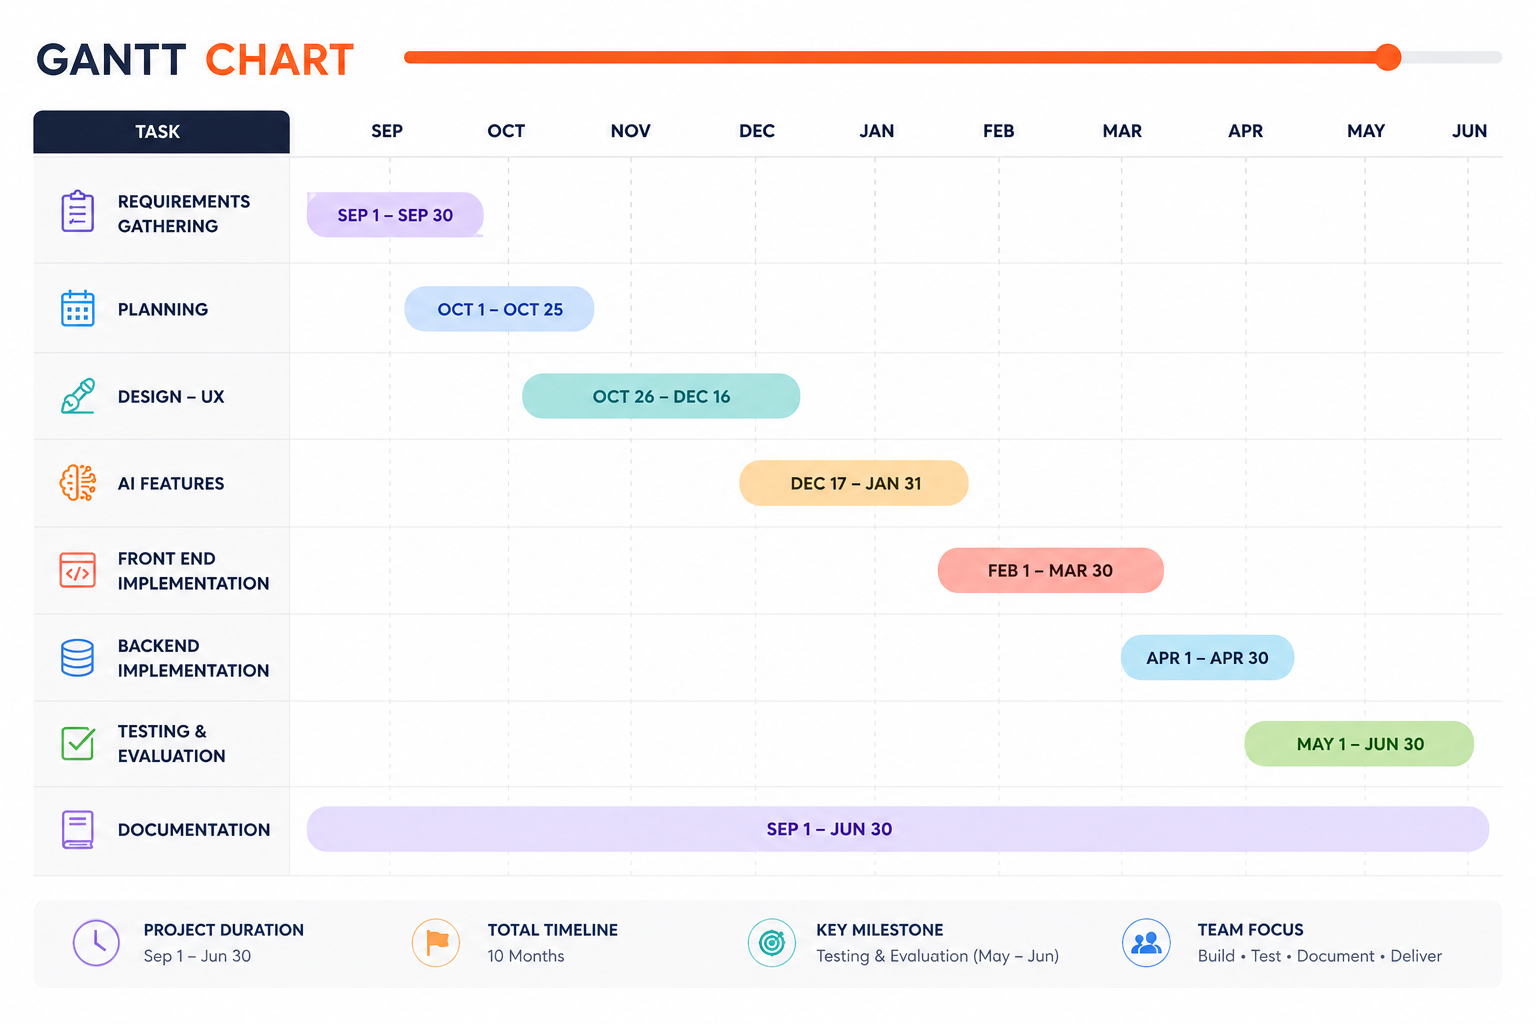
\includegraphics[width=0.95\linewidth,height=0.72\textheight,keepaspectratio]{images/img_033.png}
\caption{Project Timeline Gantt Chart}
\label{fig:chapter7-project-timeline}
\end{figure}

The timeline supported iterative development. When a module produced unexpected results, adjustments were made before moving to the next integration stage.

\section{Team Roles and Contributions}

VisionSafe360 required different development responsibilities, including AI development, backend development, frontend development, testing, and documentation. The work was organized by functional role so that each part of the project had clear ownership.

Table~\ref{tab:chapter7-team-roles} summarizes the main project roles and contribution areas.

\begin{table}[H]
\centering
\renewcommand{\arraystretch}{1.55}
\begin{tabular}{|>{\centering\arraybackslash}p{0.3\linewidth}|>{\centering\arraybackslash}p{0.58\linewidth}|}
\hline
\textbf{Role} & \textbf{Contribution Area} \\
\hline
\textbf{AI Model Development} & Dataset preparation, YOLO model training, pose analysis, fall rules, and hazard detection logic \\
\hline
\textbf{Backend Development} & API design, incident logging, alert management, WebSocket updates, and data handling \\
\hline
\textbf{Frontend Development} & Dashboard pages, live monitoring interface, alert views, reports, and ergonomic analytics interface \\
\hline
\textbf{Testing and Evaluation} & Test case design, model evaluation, runtime measurement, and result analysis \\
\hline
\textbf{Documentation} & Report writing, diagrams, tables, formatting, and final project organization \\
\hline
\end{tabular}
\caption{\textbf{Project roles and contribution areas}}
\label{tab:chapter7-team-roles}
\end{table}

This role-based organization helped the team work in parallel while keeping the system consistent. Integration meetings were used to combine the modules and resolve conflicts between the AI pipeline, backend services, and dashboard requirements.

\section{Risk Management}

Several risks were considered during project development. These risks included technical, operational, and documentation-related issues. Table~\ref{tab:chapter7-risk-management} presents the main risks and mitigation actions.

\begin{table}[H]
\centering
\renewcommand{\arraystretch}{1.55}
\begin{tabular}{|>{\centering\arraybackslash}p{0.28\linewidth}|>{\centering\arraybackslash}p{0.28\linewidth}|>{\centering\arraybackslash}p{0.32\linewidth}|}
\hline
\textbf{Risk} & \textbf{Impact} & \textbf{Mitigation} \\
\hline
\textbf{Low detection accuracy} & Incorrect or missed safety alerts & Improve dataset quality, tune thresholds, and apply persistence logic \\
\hline
\textbf{High false positives} & Alert fatigue for supervisors & Use confidence thresholds, cooldown periods, and temporal validation \\
\hline
\textbf{Low runtime performance} & Delayed real-time monitoring & Use GPU acceleration, optimized models, and controlled input resolution \\
\hline
\textbf{Camera perspective issues} & Inaccurate proximity estimation & Tune danger-zone thresholds and apply site-specific calibration \\
\hline
\textbf{Integration errors} & Broken communication between modules & Test APIs, backend events, and dashboard updates incrementally \\
\hline
\textbf{Privacy concerns} & Ethical and legal risk & Avoid raw video storage and apply anonymization principles \\
\hline
\end{tabular}
\caption{\textbf{Project risks and mitigation actions}}
\label{tab:chapter7-risk-management}
\end{table}

Risk management was important because VisionSafe360 is a safety-related system. The system must avoid both missed hazards and excessive false alarms, since both can reduce trust in the platform.

\section{Ethical and Legal Considerations}

VisionSafe360 processes workplace video streams, which makes ethics and privacy important parts of the project. The system is designed to support worker safety, not to monitor workers for punishment or unnecessary surveillance.

The main ethical principle is that the system should be used as a safety assistant for hazard prevention and faster response. Alerts should help HSE engineers and supervisors reduce risk, improve compliance, and prevent injuries. The system should not be used to unfairly evaluate workers without clear policies and proper communication.

Privacy was considered throughout the design. The project follows the principle of minimizing stored personal data. Raw video storage is avoided, and only safety-related metadata, alerts, and selected evidence snapshots should be stored when required. In a real deployment, face blurring or anonymization should be applied before saving or transmitting any visual evidence.

Legal considerations include compliance with workplace safety regulations, data protection requirements, and organizational camera-use policies. Workers should be informed that AI-assisted monitoring is used for safety purposes. Access to incident records should be restricted based on user roles, and sensitive evidence should be protected using secure authentication and encrypted communication.

Table~\ref{tab:chapter7-ethics} summarizes the main ethical and legal controls considered in the project.

\begin{table}[H]
\centering
\renewcommand{\arraystretch}{1.55}
\begin{tabular}{|>{\centering\arraybackslash}p{0.32\linewidth}|>{\centering\arraybackslash}p{0.56\linewidth}|}
\hline
\textbf{Area} & \textbf{Control} \\
\hline
\textbf{Privacy} & Avoid continuous raw video storage and keep only necessary safety records \\
\hline
\textbf{Anonymization} & Apply face blurring or identity protection before storing visual evidence \\
\hline
\textbf{Transparency} & Inform workers that the system is used for safety monitoring and incident prevention \\
\hline
\textbf{Access Control} & Limit dashboard and incident access based on user roles \\
\hline
\textbf{Data Security} & Use secure communication and protected storage for sensitive records \\
\hline
\textbf{Fair Use} & Use alerts for corrective safety actions rather than unfair worker punishment \\
\hline
\end{tabular}
\caption{\textbf{Ethical and legal controls}}
\label{tab:chapter7-ethics}
\end{table}

These controls help ensure that the system improves workplace safety while respecting privacy, fairness, and responsible AI use.

\section{Sustainability and Societal Impact}

VisionSafe360 contributes to sustainability by improving occupational safety and reducing preventable workplace injuries. Safer workplaces reduce downtime, medical costs, equipment damage, and operational disruption. The system also supports preventive safety practices by identifying risks before they become serious incidents.

The ergonomic analysis module has a long-term societal benefit because musculoskeletal injuries often develop slowly and may not be reported immediately. By monitoring posture trends, HSE teams can identify risky tasks, redesign workflows, and reduce long-term worker health problems.

From an environmental and economic perspective, the system is designed to work with existing CCTV infrastructure. This reduces the need for specialized hardware and allows organizations to reuse cameras already installed in industrial sites. Edge processing also reduces the amount of video data sent over networks, lowering bandwidth usage and improving privacy.

Table~\ref{tab:chapter7-sustainability} summarizes the sustainability and societal impact of the project.

\begin{table}[H]
\centering
\renewcommand{\arraystretch}{1.55}
\begin{tabular}{|>{\centering\arraybackslash}p{0.32\linewidth}|>{\centering\arraybackslash}p{0.56\linewidth}|}
\hline
\textbf{Impact Area} & \textbf{Contribution} \\
\hline
\textbf{Worker Safety} & Faster detection of PPE violations, falls, and unsafe proximity events \\
\hline
\textbf{Health Protection} & Early identification of ergonomic posture risks and harmful repeated movements \\
\hline
\textbf{Economic Benefit} & Reduced accident costs, downtime, and manual reporting effort \\
\hline
\textbf{Environmental Benefit} & Reuse of existing camera infrastructure and reduced need for additional sensors \\
\hline
\textbf{Operational Sustainability} & Scalable modular design that can be expanded to more cameras and sites \\
\hline
\textbf{Social Responsibility} & Supports a safer working culture and proactive hazard prevention \\
\hline
\end{tabular}
\caption{\textbf{Sustainability and societal impact}}
\label{tab:chapter7-sustainability}
\end{table}

Overall, VisionSafe360 supports safer industrial operations and encourages a shift from reactive incident handling to proactive risk prevention.

\section{Chapter Summary}

This chapter discussed project management, team organization, risks, ethical considerations, and sustainability aspects of VisionSafe360. The work breakdown structure and timeline showed how the project was organized from requirements analysis to final testing and documentation.

The chapter also highlighted the importance of privacy, transparency, access control, and fair use because the system works with workplace video data. Finally, the sustainability discussion showed how VisionSafe360 can support worker safety, reduce long-term health risks, and improve safety culture through AI-assisted monitoring.
